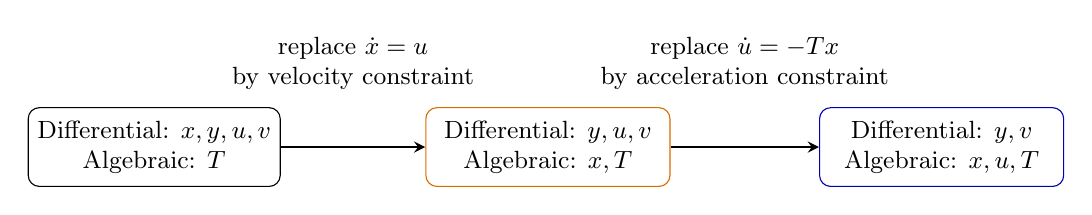
\begin{tikzpicture}[>=stealth,box/.style={draw,rounded corners,align=center,font=\small,minimum width=3.1cm,minimum height=1cm}]
\node[box](a)at(0,0){Differential: $x,y,u,v$\\Algebraic: $T$};
\node[box,draw=orange!85!black](b)at(5,0){Differential: $y,u,v$\\Algebraic: $x,T$};
\node[box,draw=blue!70!black](c)at(10,0){Differential: $y,v$\\Algebraic: $x,u,T$};
\draw[->,thick](a)--node[above=6mm,font=\small,align=center]{replace $\dot x=u$\\by velocity constraint}(b);
\draw[->,thick](b)--node[above=6mm,font=\small,align=center]{replace $\dot u=-Tx$\\by acceleration constraint}(c);
\end{tikzpicture}
